\documentclass{article}

\usepackage{noweb}
\noweboptions{smallcode,longchunks}
\usepackage[a4paper,margin=1in]{geometry}
\usepackage{colortbl}
\usepackage[colorlinks=true]{hyperref}
\usepackage{graphicx}

\newcommand{\hi}[1]{\noindent {\bf #1}}     % Define a handy paragraph opener

\def\nwendcode{\endtrivlist \endgroup}      % Remove noweb page break penalty
\let\nwdocspar=\par

\title{Jargo Communicator\footnote{
  \url{https://github.com/jargors/Communicator}}}
\author{James J. Pan\\
  \small{\href{mailto:pan-j16@mails.tsinghua.edu.cn}{pan-j16@mails.tsinghua.edu.cn}}}

\begin{document}
\maketitle
\pagestyle{noweb}

\tableofcontents

\section{Introduction}
\label{sec:introduction}
Jargo's communicator intends to be the sole way for Jargo clients to interact
with the Jargo simulated world (Figure~\ref{fig:interface-fig}). The

communicator exposes only the subset of Jargo's storage interface API that a
client would possibly have access to in the real world, including querying and
submitting server routes and schedules.  The communicator is developed using
the Noweb\footnote{\url{https://www.cs.tufts.edu/~nr/noweb/}} literate
programming\footnote{\url{http://literateprogramming.com/}} tool.  This file
({\tt{}src/Communicator.nw}) is the source for the documentation
({\tt{}doc/Communicator.tex}) and the Java code
({\tt{}Communicator.java})\footnote{See the {\tt{}Makefile} for build details.}.

\begin{figure}[h]
\centering
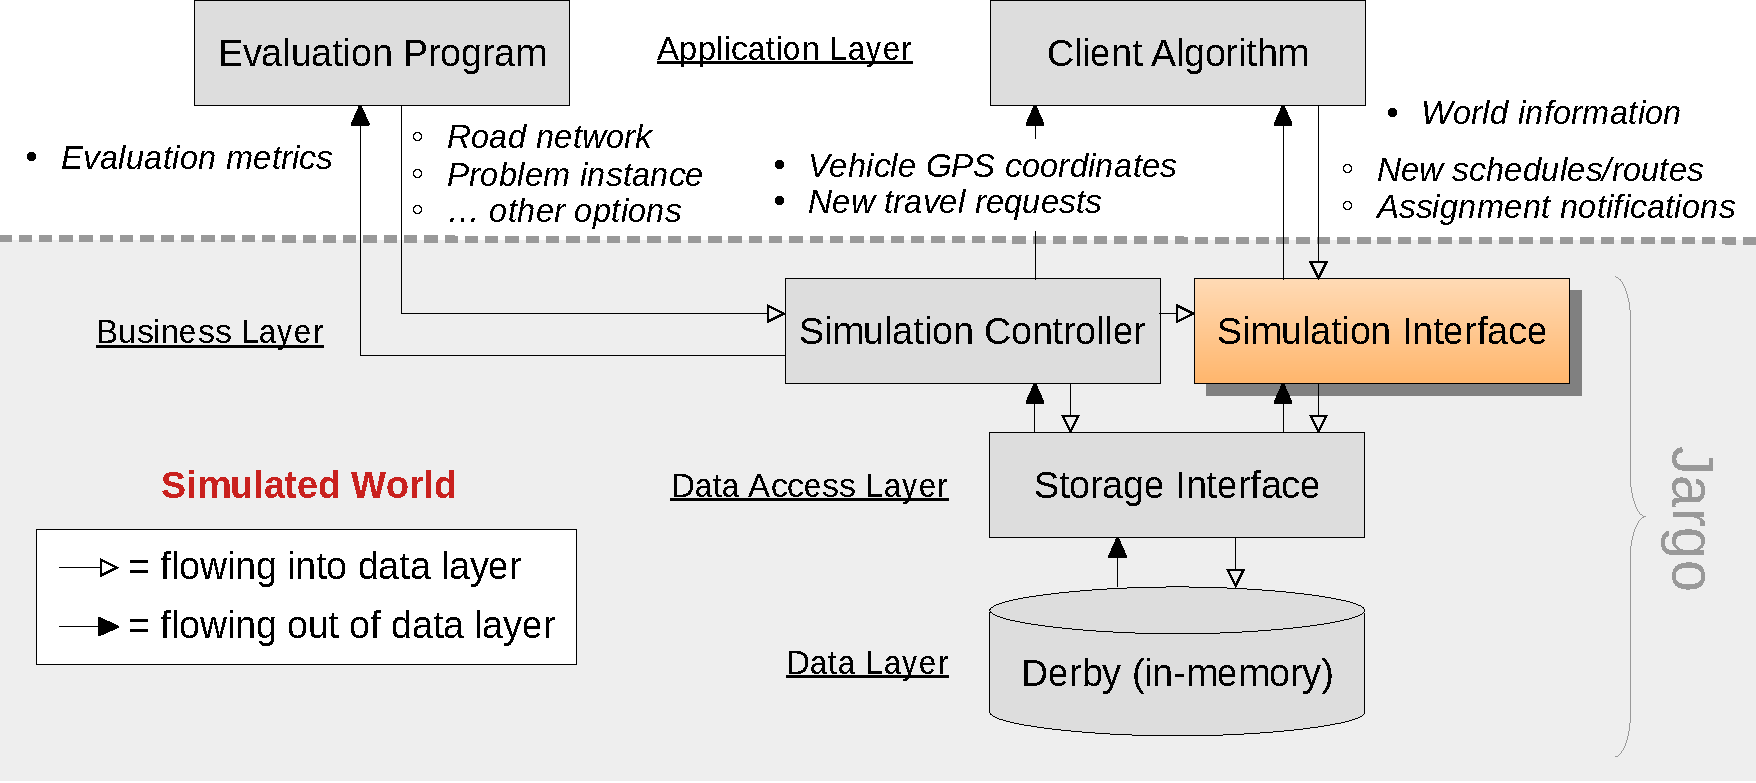
\includegraphics[width=150mm]{src/fig/interface-fig}
\caption{Communicator within the Jargo stack.}
\label{fig:interface-fig}
\end{figure}

\section{Implementation Overview}
\label{sec:implementation-overview}
\nwfilename{src/Communicator.nw}\nwbegincode{1}\sublabel{NWvbkzY-1uGZre-1}\nwmargintag{{\nwtagstyle{}\subpageref{NWvbkzY-1uGZre-1}}}\moddef{Communicator.java~{\nwtagstyle{}\subpageref{NWvbkzY-1uGZre-1}}}\endmoddef\nwnotused{Communicator.java}
\LA{}Communicator.java preamble~{\nwtagstyle{}\subpageref{NWvbkzY-3IAuyF-1}}\RA{}
\LA{}\code{}Communicator\edoc{} definition~{\nwtagstyle{}\subpageref{NWvbkzY-1DdrEr-1}}\RA{}
\nwendcode{}\nwbegindocs{2}\nwdocspar

\subsection{Preamble}
\label{sec:preamble}
The preamble declares the package and imports dependencies.
\nwenddocs{}\nwbegincode{3}\sublabel{NWvbkzY-3IAuyF-1}\nwmargintag{{\nwtagstyle{}\subpageref{NWvbkzY-3IAuyF-1}}}\moddef{Communicator.java preamble~{\nwtagstyle{}\subpageref{NWvbkzY-3IAuyF-1}}}\endmoddef\nwalsodefined{\\{NWvbkzY-3IAuyF-2}}\nwused{\\{NWvbkzY-1uGZre-1}}
package com.github.jargors;
\nwendcode{}\nwbegindocs{4}\nwdocspar
\nwenddocs{}\nwbegincode{5}\sublabel{NWvbkzY-3IAuyF-2}\nwmargintag{{\nwtagstyle{}\subpageref{NWvbkzY-3IAuyF-2}}}\moddef{Communicator.java preamble~{\nwtagstyle{}\subpageref{NWvbkzY-3IAuyF-1}}}\plusendmoddef
import com.github.jargors.Storage;
import java.util.function.Supplier;
import java.time.LocalDateTime;
import java.util.Map;
import java.util.HashMap;
\nwendcode{}\nwbegindocs{6}\nwdocspar

\subsection{Class Definition}
\label{sec:class-definition}
\nwenddocs{}\nwbegincode{7}\sublabel{NWvbkzY-1DdrEr-1}\nwmargintag{{\nwtagstyle{}\subpageref{NWvbkzY-1DdrEr-1}}}\moddef{\code{}Communicator\edoc{} definition~{\nwtagstyle{}\subpageref{NWvbkzY-1DdrEr-1}}}\endmoddef\nwused{\\{NWvbkzY-1uGZre-1}}
public class Communicator \{
  \LA{}\code{}Communicator\edoc{} member variables~{\nwtagstyle{}\subpageref{NWvbkzY-18oERh-1}}\RA{}
  \LA{}\code{}Communicator\edoc{} constructor~{\nwtagstyle{}\subpageref{NWvbkzY-1EwPlT-1}}\RA{}
  \LA{}\code{}Communicator\edoc{} public methods~{\nwtagstyle{}\subpageref{NWvbkzY-3YjONp-1}}\RA{}
  \LA{}\code{}Communicator\edoc{} private methods~{\nwtagstyle{}\subpageref{NWvbkzY-yUDLL-1}}\RA{}
\}
\nwendcode{}\nwbegindocs{8}\nwdocspar

\subsection{Member Variables}
\label{sec:member-variables}
We define a {\tt{}Storage} and a container for the simulation world time.
\nwenddocs{}\nwbegincode{9}\sublabel{NWvbkzY-18oERh-1}\nwmargintag{{\nwtagstyle{}\subpageref{NWvbkzY-18oERh-1}}}\moddef{\code{}Communicator\edoc{} member variables~{\nwtagstyle{}\subpageref{NWvbkzY-18oERh-1}}}\endmoddef\nwused{\\{NWvbkzY-1DdrEr-1}}
private Storage storage;
private int world_time = 0;
private final boolean DEBUG = false;
\nwindexdefn{storage}{storage}{NWvbkzY-18oERh-1}\nwindexdefn{world{\char95}time}{world:untime}{NWvbkzY-18oERh-1}\eatline
\nwidentdefs{\\{{storage}{storage}}\\{{world{\char95}time}{world:untime}}}\nwendcode{}\nwbegindocs{10}\nwdocspar
\subsection{Constructor}
\label{sec:constructor}
\nwenddocs{}\nwbegincode{11}\sublabel{NWvbkzY-1EwPlT-1}\nwmargintag{{\nwtagstyle{}\subpageref{NWvbkzY-1EwPlT-1}}}\moddef{\code{}Communicator\edoc{} constructor~{\nwtagstyle{}\subpageref{NWvbkzY-1EwPlT-1}}}\endmoddef\nwused{\\{NWvbkzY-1DdrEr-1}}
public Communicator() \{ \}
\nwendcode{}\nwbegindocs{12}\nwdocspar

\section{Public Methods}
\label{sec:public-methods}
\hi{General Methods.}
\nwenddocs{}\nwbegincode{13}\sublabel{NWvbkzY-3YjONp-1}\nwmargintag{{\nwtagstyle{}\subpageref{NWvbkzY-3YjONp-1}}}\moddef{\code{}Communicator\edoc{} public methods~{\nwtagstyle{}\subpageref{NWvbkzY-3YjONp-1}}}\endmoddef\nwalsodefined{\\{NWvbkzY-3YjONp-2}\\{NWvbkzY-3YjONp-3}}\nwused{\\{NWvbkzY-1DdrEr-1}}
\LA{}Set storage~{\nwtagstyle{}\subpageref{NWvbkzY-2XfZ13-1}}\RA{}
\LA{}Set/get simulation world time~{\nwtagstyle{}\subpageref{NWvbkzY-3SIXWk-1}}\RA{}
\LA{}Get reference to vertices cache~{\nwtagstyle{}\subpageref{NWvbkzY-21qmOa-1}}\RA{}
\LA{}Get reference to edges cache~{\nwtagstyle{}\subpageref{NWvbkzY-3KzwIy-1}}\RA{}
\LA{}Get reference to users cache~{\nwtagstyle{}\subpageref{NWvbkzY-1EJdXT-1}}\RA{}
\nwendcode{}\nwbegindocs{14}\nwdocspar
\hi{Write Methods.}
\nwenddocs{}\nwbegincode{15}\sublabel{NWvbkzY-3YjONp-2}\nwmargintag{{\nwtagstyle{}\subpageref{NWvbkzY-3YjONp-2}}}\moddef{\code{}Communicator\edoc{} public methods~{\nwtagstyle{}\subpageref{NWvbkzY-3YjONp-1}}}\plusendmoddef
\LA{}Update server route~{\nwtagstyle{}\subpageref{NWvbkzY-4VFddh-1}}\RA{}
\LA{}Update server add to schedule~{\nwtagstyle{}\subpageref{NWvbkzY-y828a-1}}\RA{}
\LA{}Update server remove from schedule~{\nwtagstyle{}\subpageref{NWvbkzY-lMiTm-1}}\RA{}
\nwendcode{}\nwbegindocs{16}\nwdocspar
\hi{Read Methods.}
\nwenddocs{}\nwbegincode{17}\sublabel{NWvbkzY-3YjONp-3}\nwmargintag{{\nwtagstyle{}\subpageref{NWvbkzY-3YjONp-3}}}\moddef{\code{}Communicator\edoc{} public methods~{\nwtagstyle{}\subpageref{NWvbkzY-3YjONp-1}}}\plusendmoddef
\LA{}Query vertex~{\nwtagstyle{}\subpageref{NWvbkzY-4IfXsG-1}}\RA{}
\LA{}Query edge~{\nwtagstyle{}\subpageref{NWvbkzY-1E2aru-1}}\RA{}
\LA{}Query ridesharing user~{\nwtagstyle{}\subpageref{NWvbkzY-3isdeu-1}}\RA{}
\LA{}Query active server locations~{\nwtagstyle{}\subpageref{NWvbkzY-3UaQCb-1}}\RA{}
\LA{}Query routes~{\nwtagstyle{}\subpageref{NWvbkzY-1AprqI-1}}\RA{}
\LA{}Query schedules~{\nwtagstyle{}\subpageref{NWvbkzY-3yA8FQ-1}}\RA{}
\LA{}Query remaining distance~{\nwtagstyle{}\subpageref{NWvbkzY-3tQic5-1}}\RA{}
\LA{}Query remaining duration~{\nwtagstyle{}\subpageref{NWvbkzY-2cRw59-1}}\RA{}
\LA{}Query max load~{\nwtagstyle{}\subpageref{NWvbkzY-3KLGqo-1}}\RA{}
\nwendcode{}\nwbegindocs{18}\nwdocspar

\subsection{General Methods}
\label{sec:general-methods}

\subsubsection{{\tt{}\protect\nosublabel{NWvbkzY-3YjONp-3-u9}\protect\nwindexuse{setStorage}{setStorage}{NWvbkzY-2XfZ13-1}setStorage}(1)}
\nwenddocs{}\nwbegincode{19}\sublabel{NWvbkzY-2XfZ13-1}\nwmargintag{{\nwtagstyle{}\subpageref{NWvbkzY-2XfZ13-1}}}\moddef{Set storage~{\nwtagstyle{}\subpageref{NWvbkzY-2XfZ13-1}}}\endmoddef\nwused{\\{NWvbkzY-3YjONp-1}}
public void setStorage(Storage src) \{
  storage = src;
\}
\nwindexdefn{setStorage}{setStorage}{NWvbkzY-2XfZ13-1}\eatline
\nwidentdefs{\\{{setStorage}{setStorage}}}\nwidentuses{\\{{storage}{storage}}}\nwindexuse{storage}{storage}{NWvbkzY-2XfZ13-1}\nwendcode{}\nwbegindocs{20}\nwdocspar
\subsubsection{{\tt{}\protect\nwindexuse{setSimulationWorldTime}{setSimulationWorldTime}{NWvbkzY-3SIXWk-1}setSimulationWorldTime}(1)}
We depend on the controller to tell the simulation interface about the current
world time.
\nwenddocs{}\nwbegincode{21}\sublabel{NWvbkzY-3SIXWk-1}\nwmargintag{{\nwtagstyle{}\subpageref{NWvbkzY-3SIXWk-1}}}\moddef{Set/get simulation world time~{\nwtagstyle{}\subpageref{NWvbkzY-3SIXWk-1}}}\endmoddef\nwalsodefined{\\{NWvbkzY-3SIXWk-2}}\nwused{\\{NWvbkzY-3YjONp-1}}
public void setSimulationWorldTime(int t) \{
  world_time = t;
\}
\nwindexdefn{setSimulationWorldTime}{setSimulationWorldTime}{NWvbkzY-3SIXWk-1}\eatline
\nwidentdefs{\\{{setSimulationWorldTime}{setSimulationWorldTime}}}\nwidentuses{\\{{world{\char95}time}{world:untime}}}\nwindexuse{world{\char95}time}{world:untime}{NWvbkzY-3SIXWk-1}\nwendcode{}\nwbegindocs{22}\nwdocspar
\subsubsection{{\tt{}\protect\nwindexuse{getSimulationWorldTime}{getSimulationWorldTime}{NWvbkzY-3SIXWk-2}getSimulationWorldTime}(0)}
\nwenddocs{}\nwbegincode{23}\sublabel{NWvbkzY-3SIXWk-2}\nwmargintag{{\nwtagstyle{}\subpageref{NWvbkzY-3SIXWk-2}}}\moddef{Set/get simulation world time~{\nwtagstyle{}\subpageref{NWvbkzY-3SIXWk-1}}}\plusendmoddef
public int getSimulationWorldTime() \{
  return world_time;
\}
\nwindexdefn{getSimulationWorldTime}{getSimulationWorldTime}{NWvbkzY-3SIXWk-2}\eatline
\nwidentdefs{\\{{getSimulationWorldTime}{getSimulationWorldTime}}}\nwidentuses{\\{{world{\char95}time}{world:untime}}}\nwindexuse{world{\char95}time}{world:untime}{NWvbkzY-3SIXWk-2}\nwendcode{}\nwbegindocs{24}\nwdocspar
\subsubsection{{\tt{}\protect\nwindexuse{getReferenceVerticesCache}{getReferenceVerticesCache}{NWvbkzY-21qmOa-1}getReferenceVerticesCache}(0)}
\nwenddocs{}\nwbegincode{25}\sublabel{NWvbkzY-21qmOa-1}\nwmargintag{{\nwtagstyle{}\subpageref{NWvbkzY-21qmOa-1}}}\moddef{Get reference to vertices cache~{\nwtagstyle{}\subpageref{NWvbkzY-21qmOa-1}}}\endmoddef\nwused{\\{NWvbkzY-3YjONp-1}}
public final Map<Integer, int[]> getReferenceVerticesCache() \{
  return storage.getReferenceVerticesCache();
\}
\nwindexdefn{getReferenceVerticesCache}{getReferenceVerticesCache}{NWvbkzY-21qmOa-1}\eatline
\nwidentdefs{\\{{getReferenceVerticesCache}{getReferenceVerticesCache}}}\nwidentuses{\\{{storage}{storage}}}\nwindexuse{storage}{storage}{NWvbkzY-21qmOa-1}\nwendcode{}\nwbegindocs{26}\nwdocspar
\subsubsection{{\tt{}\protect\nwindexuse{getReferenceEdgesCache}{getReferenceEdgesCache}{NWvbkzY-3KzwIy-1}getReferenceEdgesCache}(0)}
\nwenddocs{}\nwbegincode{27}\sublabel{NWvbkzY-3KzwIy-1}\nwmargintag{{\nwtagstyle{}\subpageref{NWvbkzY-3KzwIy-1}}}\moddef{Get reference to edges cache~{\nwtagstyle{}\subpageref{NWvbkzY-3KzwIy-1}}}\endmoddef\nwused{\\{NWvbkzY-3YjONp-1}}
public final Map<Integer, Map<Integer, int[]>> getReferenceEdgesCache() \{
  return storage.getReferenceEdgesCache();
\}
\nwindexdefn{getReferenceEdgesCache}{getReferenceEdgesCache}{NWvbkzY-3KzwIy-1}\eatline
\nwidentdefs{\\{{getReferenceEdgesCache}{getReferenceEdgesCache}}}\nwidentuses{\\{{storage}{storage}}}\nwindexuse{storage}{storage}{NWvbkzY-3KzwIy-1}\nwendcode{}\nwbegindocs{28}\nwdocspar
\subsubsection{{\tt{}\protect\nwindexuse{getReferenceUsersCache}{getReferenceUsersCache}{NWvbkzY-1EJdXT-1}getReferenceUsersCache}(0)}
\nwenddocs{}\nwbegincode{29}\sublabel{NWvbkzY-1EJdXT-1}\nwmargintag{{\nwtagstyle{}\subpageref{NWvbkzY-1EJdXT-1}}}\moddef{Get reference to users cache~{\nwtagstyle{}\subpageref{NWvbkzY-1EJdXT-1}}}\endmoddef\nwused{\\{NWvbkzY-3YjONp-1}}
public final Map<Integer, int[]> getReferenceUsersCache() \{
  return storage.getReferenceUsersCache();
\}
\nwindexdefn{getReferenceUsersCache}{getReferenceUsersCache}{NWvbkzY-1EJdXT-1}\eatline
\nwidentdefs{\\{{getReferenceUsersCache}{getReferenceUsersCache}}}\nwidentuses{\\{{storage}{storage}}}\nwindexuse{storage}{storage}{NWvbkzY-1EJdXT-1}\nwendcode{}\nwbegindocs{30}\nwdocspar
\subsection{Write Methods}
\label{sec:write-methods}

If the submitted route results in overwriting waypoints that a server has
already visited, in other words if {\tt{}route[0]} is less than {\tt{}\protect\nwindexuse{world{\char95}time}{world:untime}{NWvbkzY-18oERh-1}world{\char95}time},
then Communicator rejects the write. The client should be aware and handle
appropriately. To reduce rejections, ensure any submitted route does not
overwrite traveled waypoints.

\subsubsection{{\tt{}\protect\nwindexuse{updateServerRoute}{updateServerRoute}{NWvbkzY-4VFddh-1}updateServerRoute}(3)}
\nwenddocs{}\nwbegincode{31}\sublabel{NWvbkzY-4VFddh-1}\nwmargintag{{\nwtagstyle{}\subpageref{NWvbkzY-4VFddh-1}}}\moddef{Update server route~{\nwtagstyle{}\subpageref{NWvbkzY-4VFddh-1}}}\endmoddef\nwused{\\{NWvbkzY-3YjONp-2}}
public boolean updateServerRoute(int sid, int[] route, int[] sched) \{
  boolean success = false;
  if (route[0] >= world_time) \{
    storage.DBUpdateServerRoute(sid, route, sched);
    success = true;
  \}
  return success;
\}
\nwindexdefn{updateServerRoute}{updateServerRoute}{NWvbkzY-4VFddh-1}\eatline
\nwidentdefs{\\{{updateServerRoute}{updateServerRoute}}}\nwidentuses{\\{{storage}{storage}}\\{{world{\char95}time}{world:untime}}}\nwindexuse{storage}{storage}{NWvbkzY-4VFddh-1}\nwindexuse{world{\char95}time}{world:untime}{NWvbkzY-4VFddh-1}\nwendcode{}\nwbegindocs{32}\nwdocspar
\subsubsection{{\tt{}\protect\nwindexuse{updateServerAddToSchedule}{updateServerAddToSchedule}{NWvbkzY-y828a-1}updateServerAddToSchedule}(4)}
Beware, {\tt{}sched} is 3-element per stop, not 4-element like returned from the query
methods. Maybe should make consistent in the future.
\nwenddocs{}\nwbegincode{33}\sublabel{NWvbkzY-y828a-1}\nwmargintag{{\nwtagstyle{}\subpageref{NWvbkzY-y828a-1}}}\moddef{Update server add to schedule~{\nwtagstyle{}\subpageref{NWvbkzY-y828a-1}}}\endmoddef\nwused{\\{NWvbkzY-3YjONp-2}}
public boolean updateServerAddToSchedule(
    int sid, int[] route, int[] sched, int[] rid) \{
  final int t = world_time;
  final int[] current = storage.DBQueryServerRoute(sid);
  int i = 0;
  Print("Set i=0");
  Print("Set current <length>="+current.length);
  for (int q = 0; q < (current.length - 1); q += 2) \{
    System.out.print("("+current[q]+", "+current[(q + 1)]+") ");
  \}
  System.out.println();
  while (i < current.length && current[i] != route[0]) \{
    Print("Detected current["+i+"]!=route[0] ("+current[i]+"!="+route[0]+")");
    i += 2;
  \}
  Print("Got i="+i);
  if (i == current.length) \{
    // branch point not found
    Print("Branch point not found");
    return false;
  \} else \{
    Print("Found branch point at i="+i);
  \}
  int j = 0;
  while (j < route.length && route[j] <= t) \{
    if (current[i] != route[j] || current[(i + 1)] != route[(j + 1)]) \{
      // overwrite history occurred
      Print("Overwrite history detected, i="+i+", j="+j+" ("+current[i]+"!="+route[j]+", "
        +current[(i + 1)]+"!="+route[(j + 1)]+")");
      return false;
    \} else \{
      Print("Detected matching history, i="+i+", j="+j+" ("+current[i]+"="+route[j]+", "
        +current[(i + 1)]+"="+route[(j + 1)]+")");
    \}
    i += 2;
    j += 2;
  \}
  storage.DBUpdateServerAddToSchedule(sid, route, sched, rid);
  return true;
\}
\nwindexdefn{updateServerAddToSchedule}{updateServerAddToSchedule}{NWvbkzY-y828a-1}\eatline
\nwidentdefs{\\{{updateServerAddToSchedule}{updateServerAddToSchedule}}}\nwidentuses{\\{{Print}{Print}}\\{{storage}{storage}}\\{{world{\char95}time}{world:untime}}}\nwindexuse{Print}{Print}{NWvbkzY-y828a-1}\nwindexuse{storage}{storage}{NWvbkzY-y828a-1}\nwindexuse{world{\char95}time}{world:untime}{NWvbkzY-y828a-1}\nwendcode{}\nwbegindocs{34}\nwdocspar
\subsubsection{{\tt{}\protect\nwindexuse{updateServerRemoveFromSchedule}{updateServerRemoveFromSchedule}{NWvbkzY-lMiTm-1}updateServerRemoveFromSchedule}(4)}
\nwenddocs{}\nwbegincode{35}\sublabel{NWvbkzY-lMiTm-1}\nwmargintag{{\nwtagstyle{}\subpageref{NWvbkzY-lMiTm-1}}}\moddef{Update server remove from schedule~{\nwtagstyle{}\subpageref{NWvbkzY-lMiTm-1}}}\endmoddef\nwused{\\{NWvbkzY-3YjONp-2}}
public boolean updateServerRemoveFromSchedule(
    int sid, int[] route, int[] sched, int[] rid) \{
  boolean success = false;
  if (route[0] >= world_time) \{
    storage.DBUpdateServerRemoveFromSchedule(sid, route, sched, rid);
  \}
  return success;
\}
\nwindexdefn{updateServerRemoveFromSchedule}{updateServerRemoveFromSchedule}{NWvbkzY-lMiTm-1}\eatline
\nwidentdefs{\\{{updateServerRemoveFromSchedule}{updateServerRemoveFromSchedule}}}\nwidentuses{\\{{storage}{storage}}\\{{world{\char95}time}{world:untime}}}\nwindexuse{storage}{storage}{NWvbkzY-lMiTm-1}\nwindexuse{world{\char95}time}{world:untime}{NWvbkzY-lMiTm-1}\nwendcode{}\nwbegindocs{36}\nwdocspar
\subsection{Read Methods}
\label{sec:read-methods}

\subsubsection{{\tt{}\protect\nwindexuse{queryVertex}{queryVertex}{NWvbkzY-4IfXsG-1}queryVertex}(1)}
\nwenddocs{}\nwbegincode{37}\sublabel{NWvbkzY-4IfXsG-1}\nwmargintag{{\nwtagstyle{}\subpageref{NWvbkzY-4IfXsG-1}}}\moddef{Query vertex~{\nwtagstyle{}\subpageref{NWvbkzY-4IfXsG-1}}}\endmoddef\nwused{\\{NWvbkzY-3YjONp-3}}
public int[] queryVertex(int v) throws RuntimeException \{
  return storage.DBQueryVertex(v);
\}
\nwindexdefn{queryVertex}{queryVertex}{NWvbkzY-4IfXsG-1}\eatline
\nwidentdefs{\\{{queryVertex}{queryVertex}}}\nwidentuses{\\{{storage}{storage}}}\nwindexuse{storage}{storage}{NWvbkzY-4IfXsG-1}\nwendcode{}\nwbegindocs{38}\nwdocspar
\subsubsection{{\tt{}\protect\nwindexuse{queryEdge}{queryEdge}{NWvbkzY-1E2aru-1}queryEdge}(2)}
\nwenddocs{}\nwbegincode{39}\sublabel{NWvbkzY-1E2aru-1}\nwmargintag{{\nwtagstyle{}\subpageref{NWvbkzY-1E2aru-1}}}\moddef{Query edge~{\nwtagstyle{}\subpageref{NWvbkzY-1E2aru-1}}}\endmoddef\nwused{\\{NWvbkzY-3YjONp-3}}
public int[] queryEdge(int v1, int v2) throws RuntimeException \{
  return storage.DBQueryEdge(v1, v2);
\}
\nwindexdefn{queryEdge}{queryEdge}{NWvbkzY-1E2aru-1}\eatline
\nwidentdefs{\\{{queryEdge}{queryEdge}}}\nwidentuses{\\{{storage}{storage}}}\nwindexuse{storage}{storage}{NWvbkzY-1E2aru-1}\nwendcode{}\nwbegindocs{40}\nwdocspar
\subsubsection{{\tt{}\protect\nwindexuse{queryUser}{queryUser}{NWvbkzY-3isdeu-1}queryUser}(1)}
\nwenddocs{}\nwbegincode{41}\sublabel{NWvbkzY-3isdeu-1}\nwmargintag{{\nwtagstyle{}\subpageref{NWvbkzY-3isdeu-1}}}\moddef{Query ridesharing user~{\nwtagstyle{}\subpageref{NWvbkzY-3isdeu-1}}}\endmoddef\nwused{\\{NWvbkzY-3YjONp-3}}
public int[] queryUser(int uid) throws RuntimeException \{
  return storage.DBQueryUser(uid);
\}
\nwindexdefn{queryUser}{queryUser}{NWvbkzY-3isdeu-1}\eatline
\nwidentdefs{\\{{queryUser}{queryUser}}}\nwidentuses{\\{{storage}{storage}}}\nwindexuse{storage}{storage}{NWvbkzY-3isdeu-1}\nwendcode{}\nwbegindocs{42}\nwdocspar
\subsubsection{{\tt{}\protect\nwindexuse{queryServerLocationsActive}{queryServerLocationsActive}{NWvbkzY-3UaQCb-1}queryServerLocationsActive}(1)}
\nwenddocs{}\nwbegincode{43}\sublabel{NWvbkzY-3UaQCb-1}\nwmargintag{{\nwtagstyle{}\subpageref{NWvbkzY-3UaQCb-1}}}\moddef{Query active server locations~{\nwtagstyle{}\subpageref{NWvbkzY-3UaQCb-1}}}\endmoddef\nwused{\\{NWvbkzY-3YjONp-3}}
public int[] queryServerLocationsActive(int t) throws RuntimeException \{
  return storage.DBQueryServerLocationsActive(t);
\}
\nwindexdefn{queryServerLocationsActive}{queryServerLocationsActive}{NWvbkzY-3UaQCb-1}\eatline
\nwidentdefs{\\{{queryServerLocationsActive}{queryServerLocationsActive}}}\nwidentuses{\\{{storage}{storage}}}\nwindexuse{storage}{storage}{NWvbkzY-3UaQCb-1}\nwendcode{}\nwbegindocs{44}\nwdocspar
\subsubsection{{\tt{}\protect\nwindexuse{queryServerRemainingRoute}{queryServerRemainingRoute}{NWvbkzY-1AprqI-1}queryServerRemainingRoute}(2)}
\nwenddocs{}\nwbegincode{45}\sublabel{NWvbkzY-1AprqI-1}\nwmargintag{{\nwtagstyle{}\subpageref{NWvbkzY-1AprqI-1}}}\moddef{Query routes~{\nwtagstyle{}\subpageref{NWvbkzY-1AprqI-1}}}\endmoddef\nwused{\\{NWvbkzY-3YjONp-3}}
public int[] queryServerRemainingRoute(int sid, int t) throws RuntimeException \{
  return storage.DBQueryServerRemainingRoute(sid, t);
\}
\nwindexdefn{queryServerRemainingRoute}{queryServerRemainingRoute}{NWvbkzY-1AprqI-1}\eatline
\nwidentdefs{\\{{queryServerRemainingRoute}{queryServerRemainingRoute}}}\nwidentuses{\\{{storage}{storage}}}\nwindexuse{storage}{storage}{NWvbkzY-1AprqI-1}\nwendcode{}\nwbegindocs{46}\nwdocspar
\subsubsection{{\tt{}\protect\nwindexuse{queryServerRemainingSchedule}{queryServerRemainingSchedule}{NWvbkzY-3yA8FQ-1}queryServerRemainingSchedule}(2)}
\nwenddocs{}\nwbegincode{47}\sublabel{NWvbkzY-3yA8FQ-1}\nwmargintag{{\nwtagstyle{}\subpageref{NWvbkzY-3yA8FQ-1}}}\moddef{Query schedules~{\nwtagstyle{}\subpageref{NWvbkzY-3yA8FQ-1}}}\endmoddef\nwused{\\{NWvbkzY-3YjONp-3}}
public int[] queryServerRemainingSchedule(int sid, int t) throws RuntimeException \{
  return storage.DBQueryServerRemainingSchedule(sid, t);
\}
\nwindexdefn{queryServerRemainingSchedule}{queryServerRemainingSchedule}{NWvbkzY-3yA8FQ-1}\eatline
\nwidentdefs{\\{{queryServerRemainingSchedule}{queryServerRemainingSchedule}}}\nwidentuses{\\{{storage}{storage}}}\nwindexuse{storage}{storage}{NWvbkzY-3yA8FQ-1}\nwendcode{}\nwbegindocs{48}\nwdocspar
\nwenddocs{}\nwbegincode{49}\sublabel{NWvbkzY-3tQic5-1}\nwmargintag{{\nwtagstyle{}\subpageref{NWvbkzY-3tQic5-1}}}\moddef{Query remaining distance~{\nwtagstyle{}\subpageref{NWvbkzY-3tQic5-1}}}\endmoddef\nwused{\\{NWvbkzY-3YjONp-3}}
public int[] queryServerRemainingDistance(int sid, int t) throws RuntimeException \{
  return storage.DBQueryServerRemainingDistance(sid, t);
\}
\nwindexdefn{queryServerRemainingDistance}{queryServerRemainingDistance}{NWvbkzY-3tQic5-1}\eatline
\nwidentdefs{\\{{queryServerRemainingDistance}{queryServerRemainingDistance}}}\nwidentuses{\\{{storage}{storage}}}\nwindexuse{storage}{storage}{NWvbkzY-3tQic5-1}\nwendcode{}\nwbegindocs{50}\nwdocspar
\nwenddocs{}\nwbegincode{51}\sublabel{NWvbkzY-2cRw59-1}\nwmargintag{{\nwtagstyle{}\subpageref{NWvbkzY-2cRw59-1}}}\moddef{Query remaining duration~{\nwtagstyle{}\subpageref{NWvbkzY-2cRw59-1}}}\endmoddef\nwused{\\{NWvbkzY-3YjONp-3}}
public int[] queryServerRemainingDuration(int sid, int t) throws RuntimeException \{
  return storage.DBQueryServerRemainingDuration(sid, t);
\}
\nwindexdefn{queryServerRemainingDuration}{queryServerRemainingDuration}{NWvbkzY-2cRw59-1}\eatline
\nwidentdefs{\\{{queryServerRemainingDuration}{queryServerRemainingDuration}}}\nwidentuses{\\{{storage}{storage}}}\nwindexuse{storage}{storage}{NWvbkzY-2cRw59-1}\nwendcode{}\nwbegindocs{52}\nwdocspar
\subsubsection{{\tt{}\protect\nwindexuse{queryServerMaxLoad}{queryServerMaxLoad}{NWvbkzY-3KLGqo-1}queryServerMaxLoad}(2)}
\nwenddocs{}\nwbegincode{53}\sublabel{NWvbkzY-3KLGqo-1}\nwmargintag{{\nwtagstyle{}\subpageref{NWvbkzY-3KLGqo-1}}}\moddef{Query max load~{\nwtagstyle{}\subpageref{NWvbkzY-3KLGqo-1}}}\endmoddef\nwused{\\{NWvbkzY-3YjONp-3}}
public int[] queryServerMaxLoad(int sid, int t) throws RuntimeException \{
  return storage.DBQueryServerMaxLoad(sid, t);
\}
\nwindexdefn{queryServerMaxLoad}{queryServerMaxLoad}{NWvbkzY-3KLGqo-1}\eatline
\nwidentdefs{\\{{queryServerMaxLoad}{queryServerMaxLoad}}}\nwidentuses{\\{{storage}{storage}}}\nwindexuse{storage}{storage}{NWvbkzY-3KLGqo-1}\nwendcode{}\nwbegindocs{54}\nwdocspar
\section{Private Methods}
\label{sec:private-methods}

\subsection{{\tt{}\protect\nwindexuse{Print}{Print}{NWvbkzY-yUDLL-1}Print}(1)}
\nwenddocs{}\nwbegincode{55}\sublabel{NWvbkzY-yUDLL-1}\nwmargintag{{\nwtagstyle{}\subpageref{NWvbkzY-yUDLL-1}}}\moddef{\code{}Communicator\edoc{} private methods~{\nwtagstyle{}\subpageref{NWvbkzY-yUDLL-1}}}\endmoddef\nwused{\\{NWvbkzY-1DdrEr-1}}
private void Print(String msg) \{
  if (DEBUG) \{
    System.out.println("[Jargo][Communicator]["+LocalDateTime.now()+"] "+msg);
  \}
\}
\nwindexdefn{Print}{Print}{NWvbkzY-yUDLL-1}\eatline
\nwidentdefs{\\{{Print}{Print}}}\nwendcode{}

\nwixlogsorted{c}{{\code{}Communicator\edoc{} constructor}{NWvbkzY-1EwPlT-1}{\nwixu{NWvbkzY-1DdrEr-1}\nwixd{NWvbkzY-1EwPlT-1}}}%
\nwixlogsorted{c}{{\code{}Communicator\edoc{} definition}{NWvbkzY-1DdrEr-1}{\nwixu{NWvbkzY-1uGZre-1}\nwixd{NWvbkzY-1DdrEr-1}}}%
\nwixlogsorted{c}{{\code{}Communicator\edoc{} member variables}{NWvbkzY-18oERh-1}{\nwixu{NWvbkzY-1DdrEr-1}\nwixd{NWvbkzY-18oERh-1}}}%
\nwixlogsorted{c}{{\code{}Communicator\edoc{} private methods}{NWvbkzY-yUDLL-1}{\nwixu{NWvbkzY-1DdrEr-1}\nwixd{NWvbkzY-yUDLL-1}}}%
\nwixlogsorted{c}{{\code{}Communicator\edoc{} public methods}{NWvbkzY-3YjONp-1}{\nwixu{NWvbkzY-1DdrEr-1}\nwixd{NWvbkzY-3YjONp-1}\nwixd{NWvbkzY-3YjONp-2}\nwixd{NWvbkzY-3YjONp-3}}}%
\nwixlogsorted{c}{{Communicator.java}{NWvbkzY-1uGZre-1}{\nwixd{NWvbkzY-1uGZre-1}}}%
\nwixlogsorted{c}{{Communicator.java preamble}{NWvbkzY-3IAuyF-1}{\nwixu{NWvbkzY-1uGZre-1}\nwixd{NWvbkzY-3IAuyF-1}\nwixd{NWvbkzY-3IAuyF-2}}}%
\nwixlogsorted{c}{{Get reference to edges cache}{NWvbkzY-3KzwIy-1}{\nwixu{NWvbkzY-3YjONp-1}\nwixd{NWvbkzY-3KzwIy-1}}}%
\nwixlogsorted{c}{{Get reference to users cache}{NWvbkzY-1EJdXT-1}{\nwixu{NWvbkzY-3YjONp-1}\nwixd{NWvbkzY-1EJdXT-1}}}%
\nwixlogsorted{c}{{Get reference to vertices cache}{NWvbkzY-21qmOa-1}{\nwixu{NWvbkzY-3YjONp-1}\nwixd{NWvbkzY-21qmOa-1}}}%
\nwixlogsorted{c}{{Query active server locations}{NWvbkzY-3UaQCb-1}{\nwixu{NWvbkzY-3YjONp-3}\nwixd{NWvbkzY-3UaQCb-1}}}%
\nwixlogsorted{c}{{Query edge}{NWvbkzY-1E2aru-1}{\nwixu{NWvbkzY-3YjONp-3}\nwixd{NWvbkzY-1E2aru-1}}}%
\nwixlogsorted{c}{{Query max load}{NWvbkzY-3KLGqo-1}{\nwixu{NWvbkzY-3YjONp-3}\nwixd{NWvbkzY-3KLGqo-1}}}%
\nwixlogsorted{c}{{Query remaining distance}{NWvbkzY-3tQic5-1}{\nwixu{NWvbkzY-3YjONp-3}\nwixd{NWvbkzY-3tQic5-1}}}%
\nwixlogsorted{c}{{Query remaining duration}{NWvbkzY-2cRw59-1}{\nwixu{NWvbkzY-3YjONp-3}\nwixd{NWvbkzY-2cRw59-1}}}%
\nwixlogsorted{c}{{Query ridesharing user}{NWvbkzY-3isdeu-1}{\nwixu{NWvbkzY-3YjONp-3}\nwixd{NWvbkzY-3isdeu-1}}}%
\nwixlogsorted{c}{{Query routes}{NWvbkzY-1AprqI-1}{\nwixu{NWvbkzY-3YjONp-3}\nwixd{NWvbkzY-1AprqI-1}}}%
\nwixlogsorted{c}{{Query schedules}{NWvbkzY-3yA8FQ-1}{\nwixu{NWvbkzY-3YjONp-3}\nwixd{NWvbkzY-3yA8FQ-1}}}%
\nwixlogsorted{c}{{Query vertex}{NWvbkzY-4IfXsG-1}{\nwixu{NWvbkzY-3YjONp-3}\nwixd{NWvbkzY-4IfXsG-1}}}%
\nwixlogsorted{c}{{Set storage}{NWvbkzY-2XfZ13-1}{\nwixu{NWvbkzY-3YjONp-1}\nwixd{NWvbkzY-2XfZ13-1}}}%
\nwixlogsorted{c}{{Set/get simulation world time}{NWvbkzY-3SIXWk-1}{\nwixu{NWvbkzY-3YjONp-1}\nwixd{NWvbkzY-3SIXWk-1}\nwixd{NWvbkzY-3SIXWk-2}}}%
\nwixlogsorted{c}{{Update server add to schedule}{NWvbkzY-y828a-1}{\nwixu{NWvbkzY-3YjONp-2}\nwixd{NWvbkzY-y828a-1}}}%
\nwixlogsorted{c}{{Update server remove from schedule}{NWvbkzY-lMiTm-1}{\nwixu{NWvbkzY-3YjONp-2}\nwixd{NWvbkzY-lMiTm-1}}}%
\nwixlogsorted{c}{{Update server route}{NWvbkzY-4VFddh-1}{\nwixu{NWvbkzY-3YjONp-2}\nwixd{NWvbkzY-4VFddh-1}}}%
\nwixlogsorted{i}{{getReferenceEdgesCache}{getReferenceEdgesCache}}%
\nwixlogsorted{i}{{getReferenceUsersCache}{getReferenceUsersCache}}%
\nwixlogsorted{i}{{getReferenceVerticesCache}{getReferenceVerticesCache}}%
\nwixlogsorted{i}{{getSimulationWorldTime}{getSimulationWorldTime}}%
\nwixlogsorted{i}{{Print}{Print}}%
\nwixlogsorted{i}{{queryEdge}{queryEdge}}%
\nwixlogsorted{i}{{queryServerLocationsActive}{queryServerLocationsActive}}%
\nwixlogsorted{i}{{queryServerMaxLoad}{queryServerMaxLoad}}%
\nwixlogsorted{i}{{queryServerRemainingDistance}{queryServerRemainingDistance}}%
\nwixlogsorted{i}{{queryServerRemainingDuration}{queryServerRemainingDuration}}%
\nwixlogsorted{i}{{queryServerRemainingRoute}{queryServerRemainingRoute}}%
\nwixlogsorted{i}{{queryServerRemainingSchedule}{queryServerRemainingSchedule}}%
\nwixlogsorted{i}{{queryUser}{queryUser}}%
\nwixlogsorted{i}{{queryVertex}{queryVertex}}%
\nwixlogsorted{i}{{setSimulationWorldTime}{setSimulationWorldTime}}%
\nwixlogsorted{i}{{setStorage}{setStorage}}%
\nwixlogsorted{i}{{storage}{storage}}%
\nwixlogsorted{i}{{updateServerAddToSchedule}{updateServerAddToSchedule}}%
\nwixlogsorted{i}{{updateServerRemoveFromSchedule}{updateServerRemoveFromSchedule}}%
\nwixlogsorted{i}{{updateServerRoute}{updateServerRoute}}%
\nwixlogsorted{i}{{world{\char95}time}{world:untime}}%
\nwbegindocs{56}\nwdocspar
\appendix

\section{Appendix: List of Chunks}
\label{ap:list-of-chunks}
\nowebchunks

\section{Appendix: List of Identifiers}
\label{ap:list-of-identifiers}
\nowebindex

\end{document}

\nwenddocs{}
